\chapter{Results and Discussion}\label{cha:results}
\FloatBarrier

After the steps of choosing the input data, selecting the static analysis
tools, and processing their reports to generate a predictive model, the question is \emph{how well does
it work?} We now
discuss the performance of the binary prediction model trained with
AdaBoost to classify static analysis tool warnings as true or false positives and
evaluate the ranking system described in Section~\ref{subsec:ranking}.

\section{Classifier}

The data collection steps of our experiment resulted in a data set of $25,959$ labeled
warnings. To train the classifier, we divided them
into a training set with $19,470$ examples and a test set with $6,489$
examples. The former was used to train the model and tune parameters with 
10-fold cross-validation.

The final classifier was trained with 100 AdaBoost iterations ($T = 100$),
producing 100 decision trees to compose the predictive model, reaching $0.8$
mean accuracy (the proportion of correct classifications in relation to the total input)
in the cross-validation during training. This value for $T$ was
selected based on the performance of the mean accuracy of the model during training for a 10-fold
cross-validation, as can be seen in Table~\ref{tab:mean_acc}.

  \begin{table}
    \begin{center}
        \begin{tabular}{rr}\hline
          Number of trees ($T$) & Mean accuracy \\
        \hline
          10 & 0.797 \\
          50 & 0.791 \\
          \textbf{100} & \textbf{0.801} \\
          150 & 0.794 \\ \hline
        \end{tabular}
        \caption{Mean training classification accuracy (cross-validation)}\label{tab:mean_acc}
    \end{center}
\end{table}

Accuracy is just one of the interesting metrics we can derive from the experiments.
Table~\ref{tab:matrix} presents a confusion matrix for the classification of
the examples in the test set with our trained prediction model. It readily
shows the low number of misclassified labeled true positives (i.e., our model
classified real bugs correctly most of the time) and the high number of
misclassified false positives (our model classified false bugs incorrectly
more often than desirable) but, most importantly,
we can use it to calculate the classification accuracy, precision and recall for the
model over the test data set.


% confusion matrix
\begin{table}
  \begin{center}
\begin{tabular}{|c|c|c|c|c|}
\hline
                                            &                                        & \textbf{Warning}                      & \textbf{Labels}                       &                                        \\ 
                                            &                                        & TP                                    & FP                                    & \textit{Total} \\ 
                                            & TP                                     & \textbf{2440}                         & \textbf{1158}                         & \textbf{3598}  \\ 
                                            & FP                                     & \textbf{107}                          & \textbf{2784}                         & \textbf{2891}  \\ 
\multirow{-5}{*}{\textbf{Model Prediction}} & \textit{Total} & \textbf{2547} & \textbf{3942} & \textbf{6489}  \\ \hline
\end{tabular}
\caption{Confusion matrix}\label{tab:matrix}
\end{center}
\end{table}


\textbf{Accuracy (0.805)} is the number of correct classifications
    (True Positive and True Negative) divided by the total input (all
    generated warnings) and serves as a general indicator of how well
    the classifier performed. As mentioned before, our model offered an
    accuracy of 0.805 over the test set. We must recall that we cannot
    directly compare
    this accuracy metric with the accuracy of any of the tools we used:
    The definitions of what constitutes a true or false
    negative for the tools are not the same as those for the classifier.
    For the tools, a false negative involves
    sites in Juliet for which they did not trigger any warnings,
    and our model does not consider such sites. Still, we can
    compare this value with those of related works. For instance, Ruthruff et al.~\cite{ruthruff_predicting_2008} could
    identify false positive warnings with 0.85 accuracy. We consider 0.805 to
    be an excellent result given the advantages we gained by not using information extracted from
    the analyzed source code other than the static analyzers warnings
    themselves, as already discussed.

\textbf{Precision (0.678)} is the number of True Positives divided
    by the sum of True and False Positives and indicates how rare are the
    False Positives. The result obtained from our model over the test set
    was rather low when compared to the values for recall and accuracy, at
    0.678. This low value may be influenced by the unbalanced data, where
    60.7\% of the examples are on the false positive class. The unbalanced
    data, in turn, is due to the low precision of the static analysis tools
    themselves, which is 0.392 for the combined report\footnote{This is not the
    overall precision for the tools, but for the subset of warnings we could
    label according to Juliet documentation.}, as inferred from the aggregated
    tools data in Table~\ref{tab:labeled_warnings}. Figure~\ref{fig:precisions}
    compares the precision of each individual tool and the aggregate of all tools with the precision
    of our predictive model, demonstrating that it provides considerable
    improvements over them.

\textbf{Recall (0.958)} is calculated by dividing the
    number of True Positives by the total number of Positive warnings
    in the input and indicates how many Positive
    warnings in the input succeed in being recognized as such. In contrast
    to Precision, the classification recall obtained
    for the test set was considerably high: 0.958. Since we achieved such
    high recall value, if we merely pruned all warnings classified as false positives by the model,
    the loss of information (true bugs discarded) would be less than 5\%, while
    70.6\% of the noise (false alarms generated by the tools) would be discarded.

\textbf{F-score (0.794)} is the harmonic mean of Precision and Recall and
serves to present a compound view of these two other metrics, i.e., to
suggest how well the classifier performs in terms of keeping the
False Positive rate low while not discarding much of the True Positives from
the input. As we have already seen, we achieved high Recall and medium
Precision rates; the F-score value of 0.794 showcases the good performance
of the model in balancing these two goals.


\begin{figure}
\centering
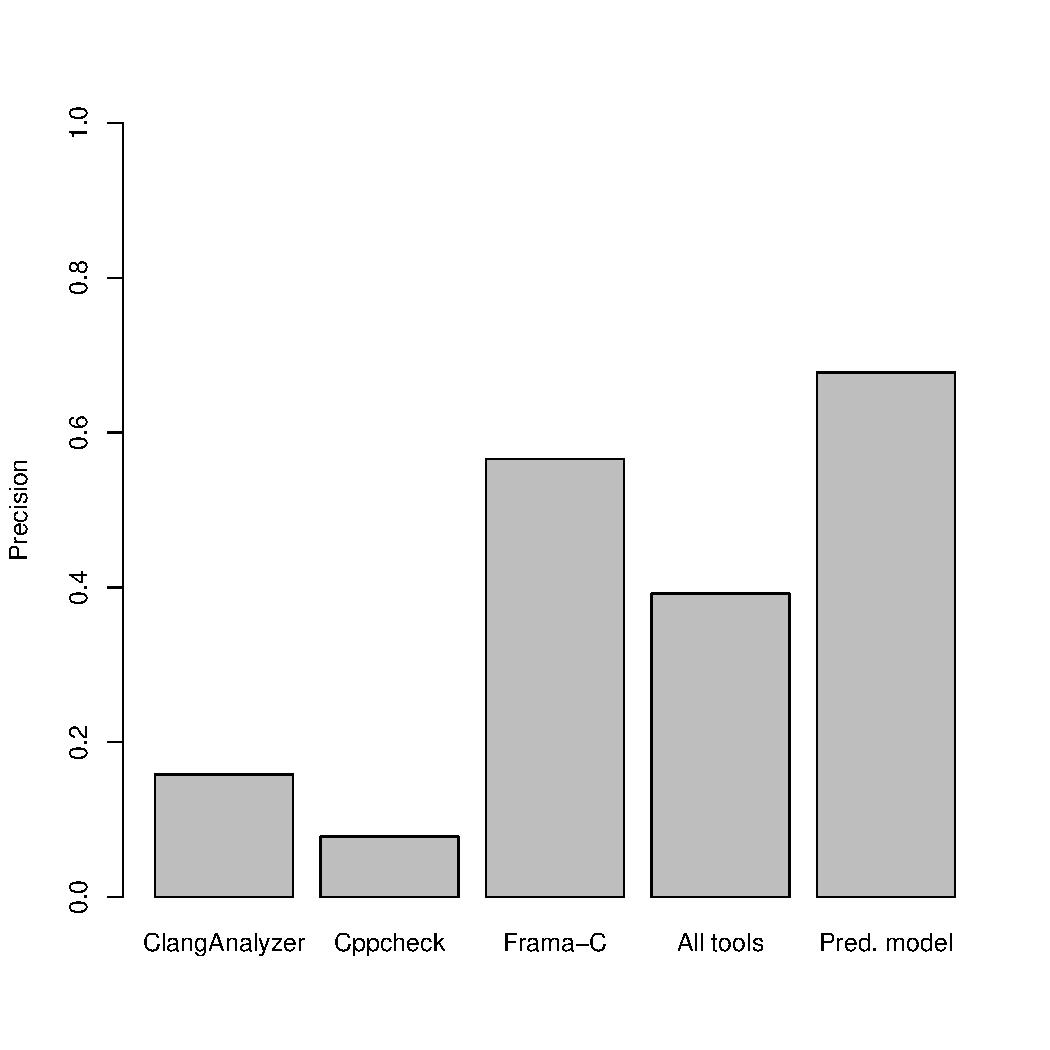
\includegraphics[width=.45\textwidth]{figures/precisions.pdf}
  \caption{Precision of each individual tool and aggregated tools (precision of all tools combined), compared with the predictive model results}\label{fig:precisions}
\end{figure}

Another aspect of interest of these results is the relevance of the features.
As discussed in Section~\ref{sec:related_work}, the most relevant features for
False Positive detection are derived from the source code itself. Since we
avoid collecting such data, which other features are the most important for
classification?  Figure~\ref{fig:feature_importance} shows that the most
relevant characteristics for classification are the total number of warnings
triggered for the file whose current warning was triggered for, the name of the
tool that triggered the warning and the confirmations of each static analyzer
for that warning. It is worth emphasizing that the feature referring to the
tool name is not independent of the 3 boolean features related to the tools
confirmations. For instance, if Cppcheck appears as the tool name for a warning,
the boolean feature for Cppcheck will be set to \emph{true}, and the other two
features, related to Frama-C and Clang Static Analyzer, will be \emph{true} if
the corresponding tool also triggers a warning for that same location and
\emph{false} if the corresponding tool does not trigger a warning for that same
location. The \emph{redundancy level} feature intent is to also capture
situations where the same tool raises more than one warning for a given
location.

%  sum of the feature importances of each individual tree, divided by the total number of trees
\begin{figure}
\centering
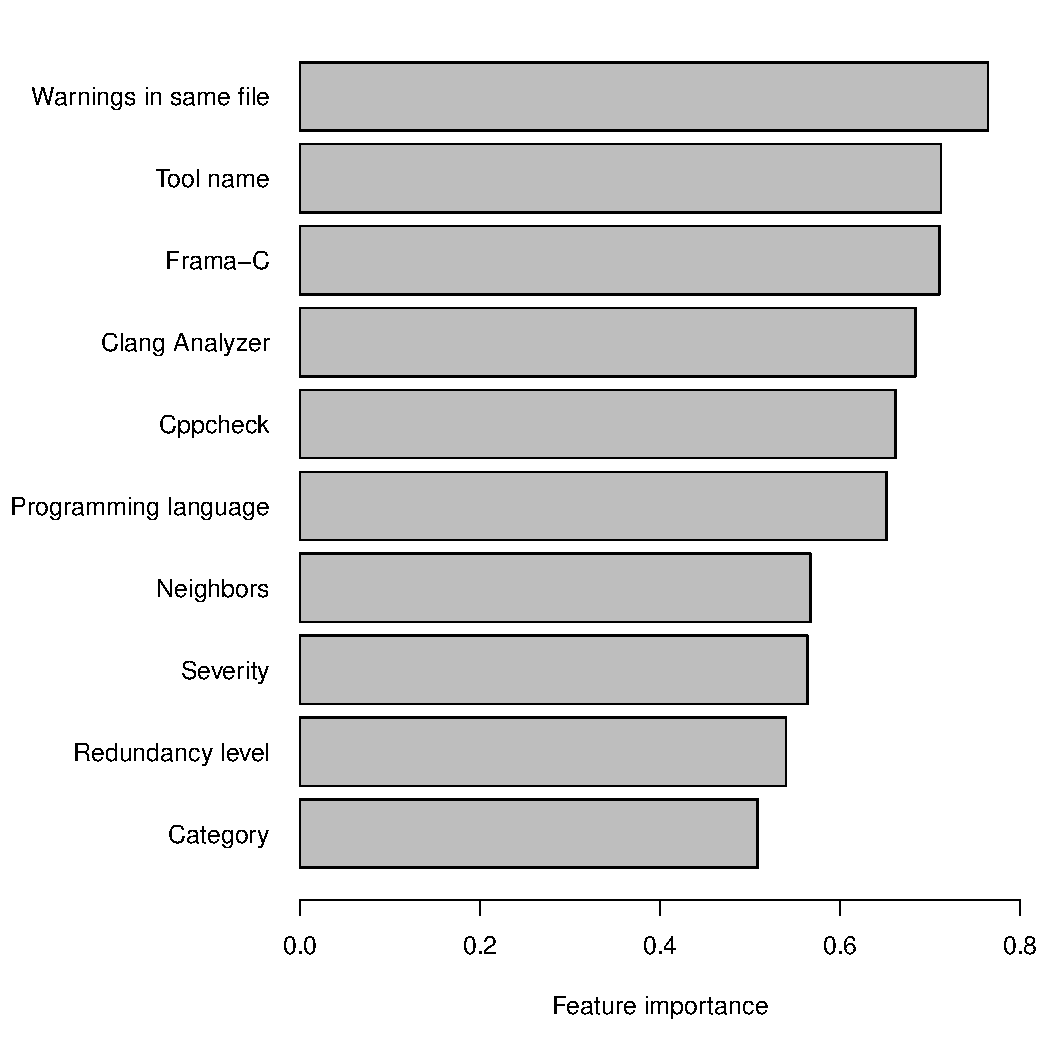
\includegraphics[width=0.45\textwidth]{figures/importance.pdf}
  \caption{AdaBoost classifier features importance: sum of the feature importances of each individual decision tree, divided by the total number of decision trees}\label{fig:feature_importance}
\end{figure}

% ranking
\section{Ranking}\label{subsection:ranking}

As mentioned before, we do not need to limit ourselves to a direct binary
classification; it is also possible to use the trained predictive model to rank
warnings according to their expected relevance. To evaluate our ranking
performance over the test set, we refer to the methodology presented by
Kremenek et al.~\cite{kremenek2004correlation}:

\begin{enumerate}

\item we define $S(R)$ to be the
sum of $FP_j$, the cumulative number of false positive warnings found before
reaching the $j_{th}$ true positive warning when navigating a ranked list
(starting from the first entry) ordered by a ranking algorithm $R$.

\begin{equation}\label{eq:sr}
  S\left(R\right) = \sum\limits_{j=1}^{N_{tp}} \mathit{FP}_j
\end{equation}

It is worth observing that $S\left(R\right) = 0$ for an optimal ranking algorithm and
$S\left(R\right) = N_{tp} \times N_{fp}$ for the worst ranking algorithm, where $N_{tp}$
and $N_{fp}$ are the total number of true positive warnings and false positive
warnings in the list, respectively.

\item We then define the average of the cumulative number of false positive
warnings found before reaching each true positive warning, $\mathit{FP}_{avg}$, as shown
in Eq.~(\ref{eq:avgfp}).

\begin{equation}\label{eq:avgfp}
  \mathit{FP}_{avg} = \frac{S\left(R\right)}{N_{tp}}
\end{equation}

\item Finally, we measure the performance ratio of our ranking algorithm against a random
ranking algorithm with Eq.~(\ref{eq:performance}).

\begin{equation}\label{eq:performance}
  \mathit{Performance} = \frac{\mathit{FP}_{avg}(\mathit{random})}{\mathit{FP}_{avg}(\text{AdaBoost ranking})}
\end{equation}

\end{enumerate}

The random ranking algorithm randomly shuffles the test set. To avoid bias in
our experiment, we run the random algorithm 10 times, calculate the
$\mathit{FP}_{avg}$ for each of them and use the median value as
$\mathit{FP}_{avg}(\mathit{random})$ to calculate the performance ratio in
Eq.~(\ref{eq:performance}). Table~\ref{tab:avgfp} summarizes the average number
of cumulative false positives hit before each true positive is found when
navigating the list from the top to the bottom for different ranking approaches
over the test set (see Eq.~\ref{eq:avgfp}).

  \begin{table}
    \begin{center}
        \begin{tabular}{|r|r|}
          \hline
          Perfect ranking & 0 \\
          \hline
          Worst case ranking &  3942 \\
          \hline
          Random ranking & 1992 \\
          \hline
          Predictive model ranking & 380 \\
          \hline
        \end{tabular}
        \caption{Average number of cumulative false positives hit before each true positive}\label{tab:avgfp}
    \end{center}
\end{table}


\begin{figure}
\centering
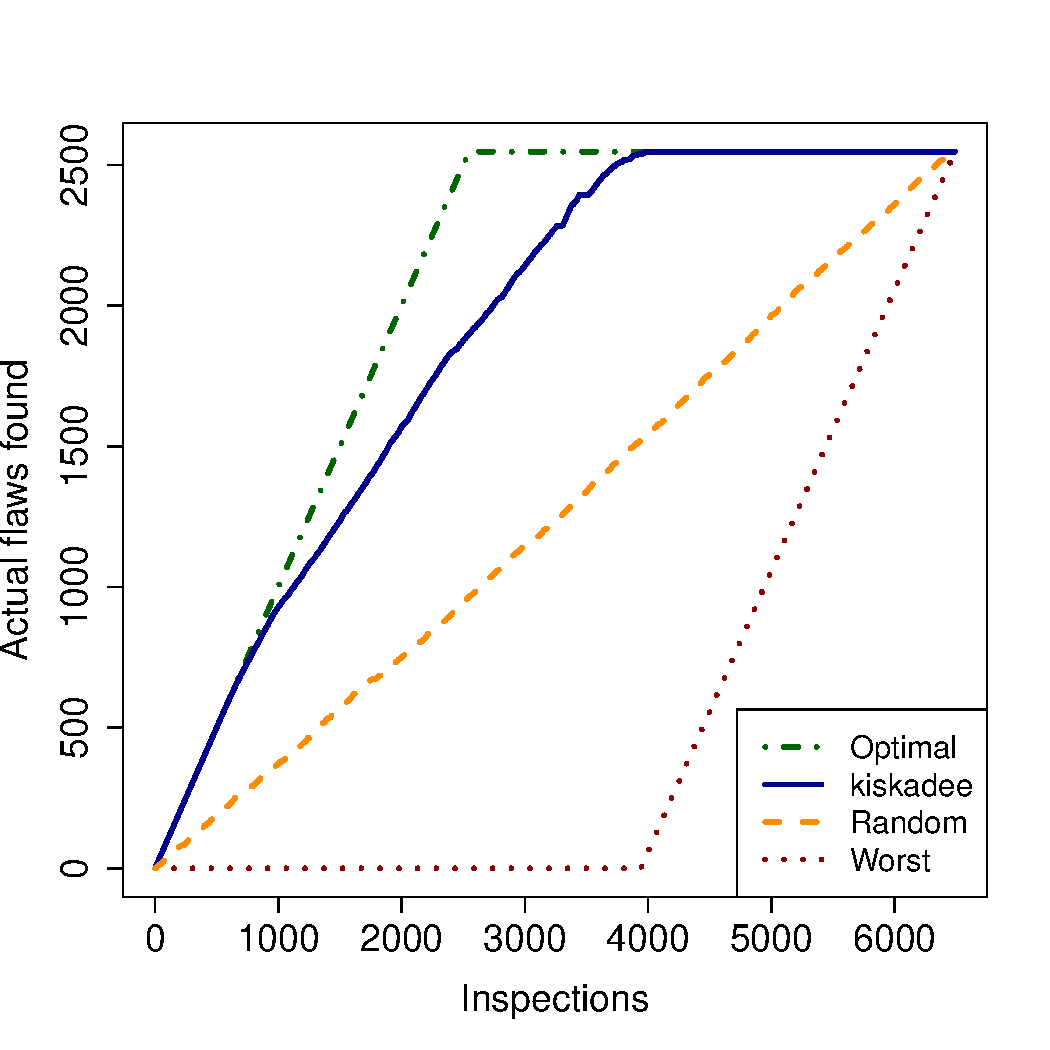
\includegraphics[width=.45\textwidth]{figures/inspections.pdf}
  \caption{Number of actual flaws hit upon top-down inspection of a ranked list for different ranking approaches. \textbf{Our Model} refers to the predictive model proposed in this study}\label{fig:inspections}
\end{figure}

The median model performance over random was $5.241$, which indicates that, on
average, one hits $5.241$ times more false positives with a random ranked
warning list than one would if using the proposed ranking.
Figure~\ref{fig:inspections} shows the number of real flaws found in a ranked
list per inspected entries (warnings) for different ranking models applied to
the test set:

\begin{itemize}
\item\textit{optimal}, where all the real flaws are in the top of the list;
\item\textit{worst}, where all the false positives are in the top of the list;
\item\textit{random}, where the entries are randomly shuffled in a list; and
\item\textit{model}, which represents the ranking model proposed in this paper while
using the classifier obtained during our experiments, as described above.
\end{itemize}

As Figure~\ref{fig:inspections} shows, our model outperforms the random ranking
algorithm by presenting all software flaws in the test set before 4000
inspections, while the random ranking algorithm presents software flaws in a
linear relation with the number of inspections, where the last few real
software flaws in the test set are only presented in the end of the list, after
6000 inspections.


\section{Discussion and Limitations}\label{sec:discussion}

As can be observed by verifying the differences between the data in
Table~\ref{tab:unlabeled_warnings} and Table~\ref{tab:labeled_warnings}, we
only used 9\% of the warnings generated by the static analysis tools over
Juliet inspections to compose our data set. We discarded the other 91\% of the
warnings generated because they were not related to the injected bugs being
tested for a given test case under analysis: they were either unintentional
flaws or false positives, and according to Juliet documentation itself, one
should not make assumptions about these warnings.

Despite this low proportion, the absolute number of warnings ($25,959$) was quite large
when compared to the sizes of data sets of similar studies. For instance, Ruthruff et
al.~\cite{ruthruff_predicting_2008} used a data set of $1,652$ warnings on
their study to predict actionable warnings. Our data set size highlights the
benefits of automatic labeling static analyzer warnings, which is only feasible
with synthetic test cases.
% I believe we can safely say that, due to undecidability of static analysis. Of course it is possible to automate the process with other means, like by analyzing bug reports for confirmed issues and matching the bug locations with the warnings, but this would still require non-trivial manual effort.

\begin{figure}
\centering
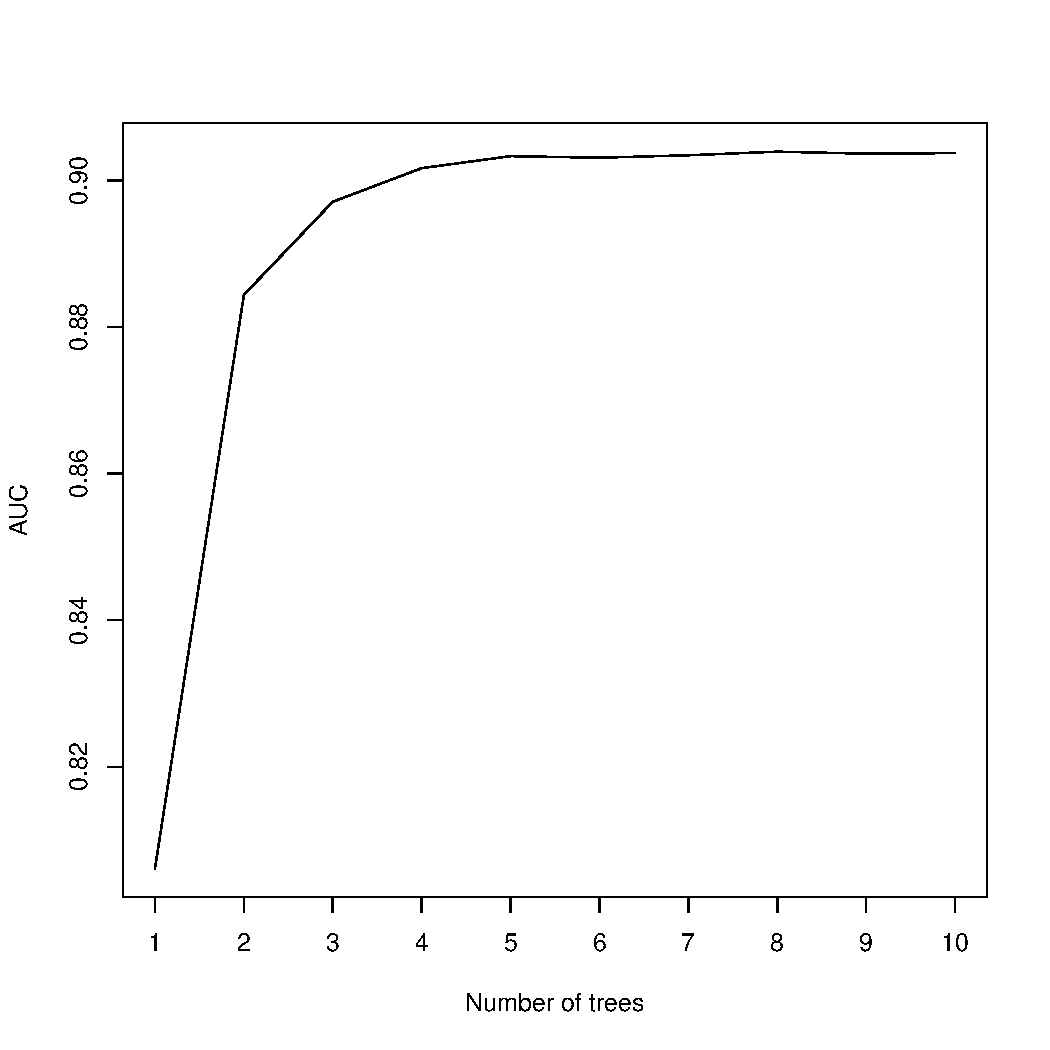
\includegraphics[width=0.45\textwidth]{figures/roc.pdf}
  \caption{Area under ROC curve versus number of trees used for AdaBoost}\label{fig:roc}
\end{figure}


Although we used $T=100$, according to the results of the cross-validation, it is
important to point out that we could not observe great variations for the
different values of $T$ we tested. Figure~\ref{fig:roc} shows how the area
under the Receiver Operating Characteristic (ROC) curve (used to compare binary
classifiers) varies as we increase the number of trees used in our model ($T$).
As can be seen, the value converges very quickly, for values of $T$ as low as 5, and remains
approximately constant up to $T = 150$, which was the highest value tested
during our experiments. At the same time, we did not observe the expected
reduction in the error rate as described in \cite{freund1999short}.
These two discrepancies in relation to the expected behavior of the weak classifiers aggregate 
could be due to the imbalance of examples present
in our data set, as can be observed in Table~\ref{tab:labeled_warnings}. This
imbalance comes from the performance of the selected static analyzers used and
might have inserted some bias in the model training experiments. Another possible
cause might be
the difficulty in classifying some examples for some specific cases. In
any case, they do not invalidate our results.

While the Accuracy, Precision, Recall, and F-Score obtained are interesting
in themselves, 
further analysis to compare the accuracy of the proposed
model to those of the static analyzers could be beneficial. We were not
able to do so because we did not collect any data
regarding the false negatives generated by the tools.

Regarding the data set used for the experiments, we relied on Juliet
1.2 documentation, provided by the US National Institute of Standards and
Technology. Thus, we performed little or no manual inspection on the warnings
triggered by the tools, meaning that any issues with the test suite or its
documentation would also lead to mislabeled examples in the data set. As
already mentioned, due to
limitations of the test suite for our purposes, we also had to
discard about 91\% of the data generated by the static analyzers. This may have
influenced the tools false positive rates, which could interfere with our model
predictions for certain flaw categories.
